\chapter{Design \label{design}}
This chapter focuses on the overall design of the solution, depicting the crucial parts. Firstly, the base system of the monitored environment. Secondly, container remotely controlled event-based monitoring of processes, file system changes and networking. Thirdly, deployment and emplacement of the isolated environment and additionally connecting it over network in a target facility or system.

\section{Specification \label{design:specs}}
This short section summarizes all specifications and assumptions considering the design. The target operating system is always Linux distribution Ubuntu 18.04.5+ with hardware enablement (HWE) or 20.04.x. The kernel specification is important for the machine hosting VMs to satisfy eBPF tools. In addition, the KVM (with QEMU) is used with the libvirt management library, which fully satisfies the choice of virtualization technology.

Regarding the VMs, there are no kernel specification, but they have Ubuntu 18.04.5+ or 20.04.x. Additionally, each VM has the minimum memory size of 4 GB and 2 virtual processors (vCPU). Although, this can vary depending of the host system resources.

\section{Environment architecture \label{design:env-arch}}
The environment has a solid underlying architecture considering a proper isolation layer and other prevention mechanisms to secure the hosting system. These operations and precautions are in compliance with the ISO 27002 standard. The bait environments within, are deliberately vulnerable in some way, therefore they are not designed to abide much of any of the ISO 27000 standards. The main goal is a mimicking production environment build atop of Kubernetes cluster. Sequentially, this section covers all in a bottom-up fashion through Kubernetes cluster design to system environments.

The considered specific control categories of the "Information technology -- Security techniques -- Code of practice for information security controls" - ISO 27002 are\footnote{All of the outlined categories are derived from the official standard \cite{iso:27002} with proper numbering preserved}:
\begin{enumerate}[label=\arabic*.,ref={ISO-27002 category \theenumi},start=12]
	\item Operations security \label{iso.12}
	\begin{enumerate}[label=\arabic*.,ref=\theenumi.\arabic*]
		\item Operational procedures and responsibilities \label{iso.12.1}
		\item Protection from malware \label{iso.12.2}
		\item Backup \label{iso.12.3}
		\item Logging and monitoring \label{iso.12.4}
		\item Control of operational software \label{iso.12.5}
	\end{enumerate}
	\item Communications security \label{iso.13}
	\begin{enumerate}[label=\arabic*.,ref=\theenumi.\arabic*]
		\item Network security management \label{iso.13.1}
	\end{enumerate}
	\item System acquisition, development and maintenance \label{iso.14}
	\begin{enumerate}[label=\arabic*.,ref=\theenumi.\arabic*,start=2]
		\item Security in development and support processes \label{iso.14.2}
	\end{enumerate}
\end{enumerate}

%12       
%- 12.1   X
%- 12.2  - slightly compliant on the host system, but not much can be done on a bait system
%- 12.3   X
%- 12.4  - all soft developed keeps a log file with metrics/data but also execution logs - monitoring with prometheus of basic linux metrics
%- 12.5  - mention semantic verionsing in monitoring (software used) + ansible like everything is pamametrized to be able to rollback
%13       X
%- 13.1   X
%14       X
%- 14.2   x

Before implementation, the whole solution including program code, configurations and operation process must be documented with proper backups in terms of these control categories. According to \ref{iso.12.1} part "12.1.1 Documented operating procedures", the solution must have a technical documentation of the operations, which means including installation, setup and configuration procedures whether they are automated or not. This category links to \ref{iso.14.2}, which discusses the security of version control systems and remote repositories used for sharing and archiving. All developed programs have a dedicated repository with no sensitive configurations, which could compromise the system. Last but not least, \ref{iso.12.3} refers to creating and maintaining proper backup procedures of valuable assets. Partly it correlates with the previous categories and only together function as secure, documented, archived and reproducible in case of any failure.

\subsection{Base system \label{design:env-arch:base}}
The lowest layer is an Ubuntu host machine with KVM virtual machines (VM). Deriving from a Kubernetes cluster design in production environment, which often isn't a single-node architecture, the base system must be a set of coexisting VMs. Choosing the right number of VMs with respect to the overall resource capacity is not in scope of this thesis. Nevertheless, there are three base VMs serving as the base of the deceiving system.

The main specification defines that all VMs are identical and configured for remote operations, have functional inter-VM communication and meet all requirements (e.g. kernel version, basic security settings, hardening). Creating multiple identical VMs can be achieved by preceding mechanisms (e.g. \textit{cloud-init}\footnote{https://github.com/canonical/cloud-init}), sharing the same image or by provisioning mechanisms (e.g. \textit{Vagrant}, \textit{Ansible}).

It depends on the implementation, but since these VMs have a static and simple setup, preceding is not necessary. This technique is fully configurable and must be automated or manually ran for each VM with deviating variables e.g. host name, IP address. This is not a complicated process, but a more suitable approach is using a shared pre-configured image combined with a dedicated tool - Vagrant for seamless provisioning and installation. KVM with libvirt and Vagrant create a "VM as code" concept efficient in provisioning, preceding and whole VM management.

% TODO: move to implementation part
% This is where Vagrant comes in place to effectively manage the creation of custom VMs. In addition to Vagrant there is also inter-VM networking and choice of virtualization provider.

\subsubsection*{Setup \label{design:env-arch:base:setup}}
Base system has several dependencies and requires a custom setup of networking and host machine altogether. As mention in \autoref{design:specs}, the host depends on QEMU, KVM and libvirt to run VMs. Additionally, the VMs are connected to a libvirt-managed management network (MGMT network) and a standard inter-VM network (NODE network) also simulating public IP address pool for the Kubernetes cluster. Both of these networks are represented as Linux network bridges and are segregated to comply with \ref{iso.13.1}.

\begin{figure}[h]
	\centering
	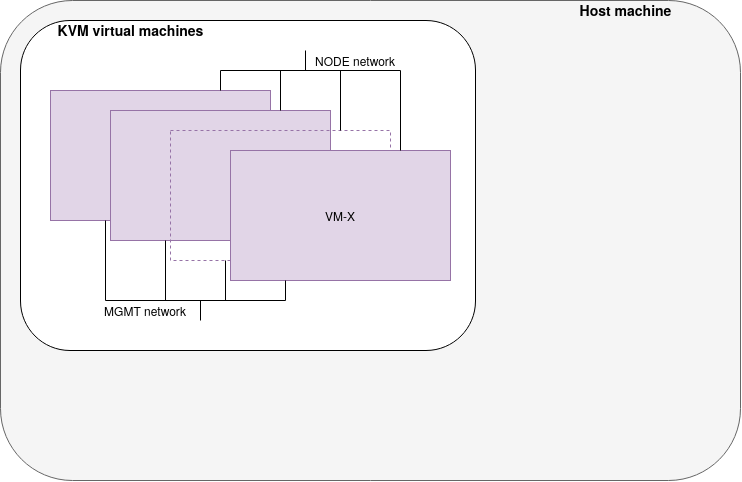
\includegraphics[scale=0.4]{base_system_design}
	\caption{Base system visualization. !!!!REVIEW ME!!!!}
	\label{image:design:base_system}
\end{figure}

Given that, the deceiving environment is isolated twice (Kubernetes-managed containers and VMs), the host machine is not expected to experience any malicious activity. Even though, a set of precautions is advised in case of any suspicious activity occurs otherwise. But only passive techniques are suitable, because all of activity from the isolated environment is routed through the host system, which must be allowed. Network security monitoring (NSM) solution designed for detection rather than prevention should effectively provide the sufficient visibility over the host system. Although, this is not the main thesis objective, so there are no specific requirements and it depends on the implementation.

\subsubsection*{Vagrant \label{design:env-arch:base:vagrant}}
Sharing a custom base image (Vagrant box), saves time on configuration and is less prone to error. Utilizing a pre-configured Vagrant box does not necessarily mean the configuration is immutable, all can be changed via Vagrant post-deploy commands and provisioning in the \textit{Vagrantfile}. Security-wise, creating a custom Vagrant box from the official Ubuntu image is recommended over publicly available Vagrant boxes from unverified owners. Not knowing the whole agenda of those boxes a full audit would be appropriate to approve their usage. Therefore, the all VMs have been created with a specific Vagrant box.

Each Vagrant box is a minimal Ubuntu (of satisfying version defined in \autoref{design:specs}) installation with the following configuration and setup:
\begin{itemize}
	\item 
	user setup including password protected \textit{root}
	\item 
	kernel parameters
	\begin{itemize}[label=$\hyphen$]
		\item
		enabled IP forwarding - \texttt{net.ipv4.ip\_forward}
	\end{itemize}
	\item 
	VM routing table entry to satisfy reverse path check - new route through the NODE network to the administration network or machine
	\item
	SSH daemon configuration
	\item 
	custom dependencies based on the implementation
\end{itemize}

Additionally everything else is done within the Vagrantfile, which is configurable with environment variables or other type of arguments. The input variables are the NODE network bridge name, IP prefix for the NODE network, number of nodes and vagrant box identifier. Altogether, the Vagrantfile creates all requested nodes as functional and remotely accessible VMs ready for Kubernetes installation and the deception environment configuration.

\subsection{Kubernetes cluster \label{design:env-arch:k8s}}
Kubernetes is complex and highly configurable, therefore a simple configuration is sufficient. There are many Kubernetes installation techniques and various derivatives meant for minimal setup and development (e.g. \textit{microk8s}\footnote{\url{https://microk8s.io/}}, \textit{minikube}\footnote{\url{https://minikube.sigs.k8s.io/docs/}}, \textit{k3s}\footnote{\url{https://k3s.io/}}). For this thesis a full Kubernetes ecosystem is preferred to mimic a production environment as much as possible.

\subsubsection*{Setup \label{design:env-arch:k8s:setup}}
Considering Kubernetes as a cloud-only platform, there are few differences to take into account when deploying microservices and applications on a bare-metal variant. Most importantly, Kubernetes is installed on those three base VMs in an arrangement of one master node with two worker nodes. Which briefly means, that the master node controls the cluster and does not provide any computational resources like the worker nodes do.

Things like storage and load balancing network traffic, are cloud provider services, which need to be substituted. Regarding persistent storage for demanding applications, the cluster is scaled up with additional dedicated node (data node) for storage. Data node is not part of the Kubernetes cluster, it serves as an external Network File System (NFS) server providing persistent storage. This node is setup in the same way as the other cluster nodes, except for the Kubernetes installation. Instead, setup with simple NFS server.

The Kubernetes ecosystem is installed via \textit{kubespray}\footnote{\url{https://kubespray.io/}}, which is a full Ansible skeleton for a complete cluster setup. Kubespray installs all dependencies, configures networking and assigns roles (master vs. worker) to all nodes. The cluster is ready for creating new objects, applications and environments.

Only after the cluster is fully functional, the before mentioned load balancing can be setup. For a bare-metal installation, the \textit{MetalLB}\footnote{\url{https://metallb.org/}} load balancer effective and provides full Kubernetes loadbalancer capabilities. MetalLB is setup in layer 2 mode, which refers to the data link layer of the RM OSI model. This mode utilizes the address discovery protocol (i.e. ARP) to route between nodes and turns one node into a point of enter. It is not a true load balancing technique, but it serves the key purpose of publishing common ports to the outside network.

\begin{figure}[h]
	\centering
	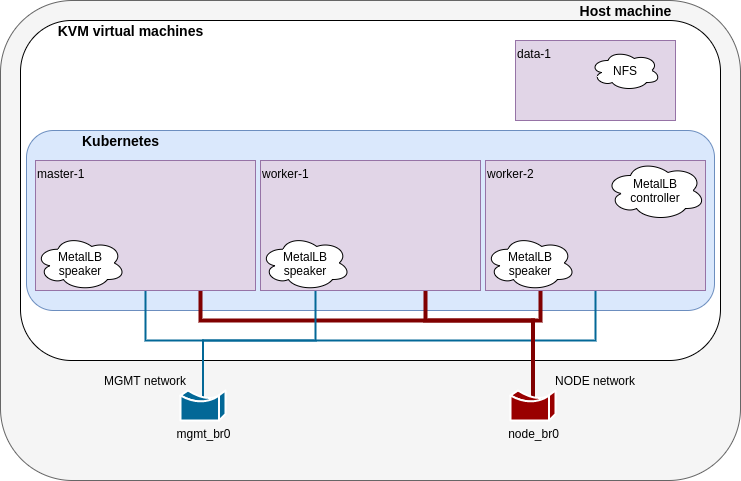
\includegraphics[scale=0.5]{k8s_design}
	\caption{Desired system setup with an environment ready Kubernetes.}
	\label{image:design:k8s}
\end{figure}

\subsubsection*{Environments \label{design:env-arch:k8s:envs}}
%mention:
%- possible environment scenarios
%- desired structure (maybe belongs to implementation)
%	- using deployments over sole pods
%	- storage class over persistent volumes
%- most of what is in the k8s-environments repo but from a design point of view
%Practically ... about the environments from architecture POV
%Technically .. about git repos and proper management for redeploying
Each environment covers a whole system with multiple applications and subsystems. In terms of Kubernetes, the environment is a collection of compatible objects/resources. Some with simple functions and dedicated applications (e.g. FTP server, private Docker registry, Gitea/GitLab, mail server or Nextcloud) others with connected active processes or dependent applications (e.g. data pipelines or microservice ecosystem). 

Technically, an environment in terms of this thesis is a collection of YAML files stored in a remote repository easily deployed to the cluster. More specifically, Kubernetes \textit{pods}, \textit{services}, configuration (via e.g. \textit{configmaps}, \textit{secrets}), mounted volumes and/or permission-related objects. Practically, pods are replaced with \textit{deployments} and published services are using service type \textit{LoadBalancer} (utilizes MetalLB).

%TODO: maybe include a design of several environments only from the application POV e.g. scenario1 - FTP + mail + blog + gitlab, scenario2 - microservice application with multiple pods ...

\section{Container monitoring \label{design:con-mon}}
Monitoring a container requires to observe container file system, networking and process execution in the most efficient way. Inspired by some related solutions, this section describes the monitoring mechanisms, tools and techniques utilized in this thesis.

\begin{itemize}
	\item 
	Points of enter, such as honeypots that lure the threat actors to the environment. Could be local to the environment or remote anywhere in the Internet.
	\item 
	3 Ubuntu server nodes are the base to Kubernetes cluster holding and orchestrating the whole environment.
	\item 
	There are to be multiple environments.
	\item
	Any environment is automated and deployed to the cluster via Ansible playbooks.
	\item 
	The core monitoring tools and programs are deployed on the hosting nodes
\end{itemize}

\subsection{Activity events \label{design:mon:events}}
The traced events, which are used to identify the malicious actor's agenda are file system, network and process related. Each type of event has a different repetition period and importance. For example, network and process events are also self-occurring (with no user initialization activity), therefore not all are held as valuable as file system changes. Files are changed less frequently and selectively choosing valuable directories, the monitoring agents gain visibility over the desired parts of the file system. Nevertheless, the down side to all types of these events are those interpreted as false positive.

According to \ref{iso.12.4} part "12.4.4 Clock synchronisation" "the clocks of all relevant information processing systems within an organization or security domain should be synchronised to a single reference time source" \cite{iso:27002}. All events are tagged with a timestamp to correctly create a timeline of all events together. Since the designed system is wrapped by VMs, which share the host machine, the time is identical each VM.

\subsubsection*{File system events \label{design:mon:events:fs}}
Any modifications or removal of existing and creation of new files in the specified locations of the file system are detected and logged. Additional events possible to monitor, are file permissions, owners, access lists and renaming. Since, "Everything is a file" mostly applies, there are expected to be many uninteresting events.

\subsubsection*{Process execution events \label{design:mon:events:proc}}
It depends on the implementation, but process events are any new instances that are readable in the output of "\texttt{ps waxu}" command. Including process and parent process IDs (PID, PPID resp.), user, command line including arguments and optionally memory and CPU usage creates an image of observed activities.

\subsubsection*{Network events \label{design:mon:events:net}}
Malicious actors use network to exfiltrate data, send commands or connect to the target service/system. Malicious programs propagate and mutate through network. For all these scenarios a different protocol or technique may be used. Although, in Kubernetes pod/container network services must be published over Kubernetes service objects, therefore setting up a backdoor listing on arbitrary port requires access to \textit{kubectl} or a vulnerability in Kubernetes itself. Meaning only existing services are of interest in addition to general exfiltration network protocols e.g. FTP, SMTP, HTTP/S, DNS, SMB according to the MITRE technique - "Exfiltration Over Alternative Protocol" \cite{mitre:T1048}.

\subsection{Tools and techniques \label{design:mon:tools}}
%- sneakpeek scripts but from a design point of view
% docker inspect output 
% bpftool, mount namespace for container segregation
% ansible or script for retrieving current setup
% templated systemd units for per-container monitoring
Whether it is monitoring from the host machine or directly from Kubernetes, a list of target containers is vital. In case of monitoring from within the containers, an agent/daemon is predefined as part of the pod in its object definition. On the other hand, for a host-based monitoring some kind of reconnaissance must occur to identify all targets in an automated way. The designed tools are described in depth in the following sections.

\subsubsection*{Host-based monitoring \label{design:mon:tools:host}}
% simple API for process monitoring of processes and systemd units
All events are detectable, to some extend, from the host. Since all activity originates from a Docker container, by design the file system, processes and network traffic is accessible.

Firstly, dynamically getting all the active containers is crucial for inspecting any of the discussed events. Using the control tool \textit{kubectl} get the cluster nodes, which host the pods. Combining \textit{kubectl} and \textit{docker-inspect}, it is simple to retrieve all containers and additional metadata. Altogether the designed tool maps all application containers to nodes for further processing.

Docker container metadata provide all the necessary information to locate the container root directory and mounted file systems. Using a standardized technique, these directories or selective subdirectories may be actively monitored for changes. More specifically, '\texttt{.[0].GraphDriver.Data.MergedDir}'\footnote{\label{footnote:jq}jq filter} gives the top level file system of the \textit{overlayfs} and '\texttt{.[0].Mounts[].Source}'$^{\ref{footnote:jq}}$ returns the mounted directories located on the host. This tool extension executes file system monitoring for each container utilizing tools like \textit{fswatch}, \textit{inotify} or \textit{opensnoop}.

Detecting executed processes is a more sofisticated issue, but using the right technique is important. eBPF enables the tool \textit{execsnoop} to tap into the kernel and record system calls. Fortunately, execsnoop allows various filtering options. Specifically the mount namespace efficiently isolates the observable system calls within a single container. For execsnoop the mount namespace identifier is shared over the BPF map objects using \textit{bpftool}, which are available for a latest kernel version requirement mentioned in \autoref{design:specs}.

Last of the event types - network traffic monitoring is much more intuitive and native to the architecture and technology used. Since the applications within the cluster are virtualized, the pod network interfaces can be traced to host accessible interfaces. Consequently, a tool taps on to the interface and effectively scans the whole traffic including a pod-to-pod and pod-to-external communications. This leaves open possibilities to tools like \textit{DPDK} or netflow collectors like \textit{suricata}, Although the design expects many pods with many interfaces, so the network traffic collector should have a minimal overhead. % TODO: add the packet capture tool used

\subsubsection*{Control tool \label{design:mon:tools:main}}
The main control (\textit{API server}) tool is for managing and controlling all of the above mentioned tools and functionality. It is a centralized API server, which has access to the execsnoop, fswatch and nettool (\textbf{TODO change}) for basic management. Additionally, API server provides additional threat hunting functionality such as:
\begin{itemize}
	\item running process information
	\item file information \textbf{MUST IMPLEMENT}
	\item \textbf{TODO other}
	% todo: !!!
\end{itemize}

\subsubsection*{Kubernetes monitoring \label{design:mon:tools:k8s}}
% service mesh - istio (SHOULD also be in analysis)
% prometheus
The minimal monitoring of the whole cluster is an ideal job for the \textit{Prometheus} toolkit combined with \textit{Grafana} dashboards for visualization. Prometheus provides visibility of the golden metrics\footnote{"Golden metrics (or “golden signals”) are the top-line metrics that you need to have an idea of whether your application is up and running as expected."\cite{goldenmetrics}}.

Apart from the network and pod monitoring, other events are not being tracked from within the cluster.

\section{Deployment and emplacement \label{design:deployment}}
This section focuses on the design of deployment methods and ideal emplacement of the system. The focus is mainly on \textit{Ansible}, \textit{Vagrant}, \textit{kubespray} and \textit{kubectl}. The main goal is an Ansible skeleton with playbooks and roles and applicable division by hosts in custom inventory(s).

\subsection{Deployment \label{design:deployment:deploy}}
The prerequisite are cluster nodes, which are deployed and pre-configured using Vagrant as discussed in \autoref{design:env-arch:base:vagrant}. While the Vagrantfile defines cluster nodes, Ansible executes scripts, additional configuration and provisioning of Kubernetes and installation of tools' dependencies.

Following the Ansible design patterns, any compact deployment is packed in an Ansible playbook or Ansible role. \autoref{design:env-arch:k8s:setup} already addresses kubespray as the Kubernetes deployment mechanism, which is not integrated to the main Ansible skeleton.

Apart from the Kubernetes deployment all required setups (both Kubernetes-related and not) and tools are provisioned by playbooks or roles. Each is fully configurable by Ansible group and host variables, which define a specific environment setup and can be cloned to configure an environment with different properties.

\subsection{Emplacement \label{design:deployment:place}}
An abstract visualization in \autoref{image:design:abstract} shows the bait system behind a firewall next to a organization's production environment. This one of possible emplacements of the system in a network. 

\begin{figure}[h]
	\centering
	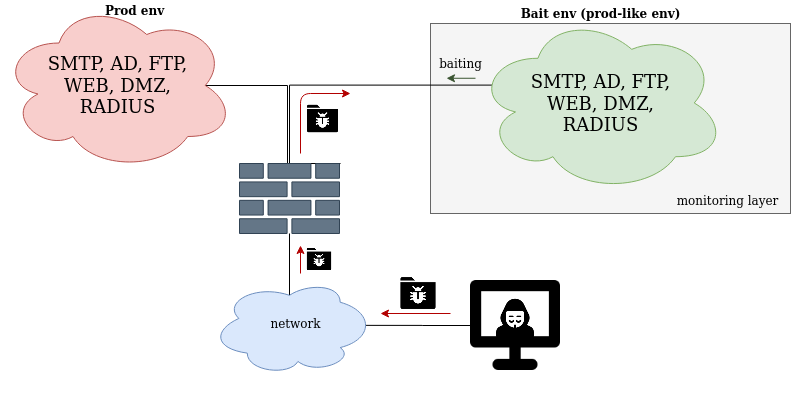
\includegraphics[scale=0.4]{abstract_diagram}
	\caption{Abstract idea of this thesis system emplacement.}
	\label{image:design:abstract}
\end{figure}

